\documentclass[tikz, preview]{standalone}
\usepackage{amsfonts, amsthm, amssymb, amsmath, stmaryrd, etoolbox}
\usepackage{tikz}
\usetikzlibrary{matrix,arrows}
\begin{document}
%%%%%%%%%%%%%%%%%	
%%%%%%%%%%%%%%%%%
\[
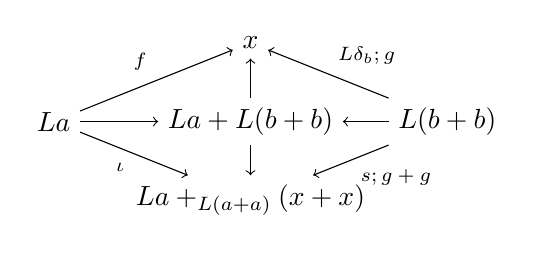
\begin{tikzpicture}
%	\draw [help lines, step=0.2, color=blue!10] (-5,-5) grid (5,5); % grid
	%
	\node (l) at (-2.5,0) {$ La $};
	\node (m1) at (0,1) {$ x $};
	\node (m2) at (0,0) {$ La + L(b+b) $};
	\node (m3) at (0,-1) {$ La +_{L(a+a)} (x+x) $};
	\node (r) at (2.5,0) {$ L(b+b) $};
	%
	\draw [->] (l) to node [above left] {\scriptsize $ f $} (m1);
	\draw [->] (l) to node [] {\scriptsize $  $} (m2);
	\draw [->] (l) to node [below left] {\scriptsize $ \iota $} (m3);
	\draw [->] (m2) to node [] {\scriptsize $  $} (m1);
	\draw [->] (m2) to node [] {\scriptsize $  $} (m3);
	\draw [->] (r) to node [above right] {\scriptsize $ L\delta_b ; g$} (m1);
	\draw [->] (r) to node [] {\scriptsize $   $} (m2);
	\draw [->] (r) to node [below right] {\scriptsize $ s ; g+g $} (m3);
\end{tikzpicture}
\]
%%%%%%%%%%%%%%%%%
%%%%%%%%%%%%%%%%%
\end{document}
